\documentclass[11pt,a4paper]{article}
\usepackage[margin=2.5cm]{geometry}
\usepackage{amsmath,amssymb,amsthm}
\usepackage{physics}
\usepackage{booktabs}
\usepackage{hyperref}
\usepackage{tikz}
\usetikzlibrary{arrows.meta,positioning,shapes.geometric,fit,backgrounds}

\newcommand{\Rxi}{R_\xi}
\newcommand{\Mpl}{M_{\mathrm{Pl}}}
\newcommand{\Mfive}{M_5}
\newcommand{\MZ}{M_Z}
\newcommand{\MW}{M_W}
\newcommand{\vEW}{v_{\mathrm{EW}}}
\newcommand{\calI}{\mathcal{I}}
\newcommand{\GN}{G_N}

\title{EDC BLOCK-003 Gravity Sector:\\
Closure Summary under Minimal Calibration}
\author{EDC Collaboration\\[3pt]
\small\textit{Program note / consolidation; no new results}}
\date{February 2026}

\begin{document}
\maketitle

\begin{abstract}
This note consolidates derivations v13--v17 into a single reader-friendly summary
of the BLOCK-003 gravity sector closure. We present the canonical derivation chain,
numerical results, robustness checks, and an explicit ``reader contract'' specifying
what is derived [D], what is identified [I], and what remains baseline-calibrated [BL].
\textbf{No new results are claimed}; this is a consolidation document.
\end{abstract}

%═══════════════════════════════════════════════════════════════════════════════
\section{Scope and Reader Contract}
%═══════════════════════════════════════════════════════════════════════════════

This document establishes a clear epistemic contract between EDC and the reader
regarding the gravity sector:

\begin{itemize}
\item \textbf{What is derived [D]:}
The 5D-to-4D reduction formula $\Mpl^2 = \Mfive^3 \calI$ follows from standard
Kaluza-Klein dimensional reduction applied to the EDC 5D Einstein-Hilbert action.
This is mathematical physics, not phenomenological fitting.

\item \textbf{What is identified [I]:}
The compactification scale $\Rxi$ is \emph{identified} with an electroweak length
scale via $\Rxi = \hbar c / \MZ^{\mathrm{obs}}$. This identification is physically
motivated but not derived from EDC axioms.

\item \textbf{What is baseline-calibrated [BL]:}
Two measured quantities serve as baseline inputs: the 4D Planck mass
$\Mpl^{\mathrm{obs}} = 1.221 \times 10^{19}$~GeV and the Z boson mass
$\MZ^{\mathrm{obs}} = 91.1876$~GeV. These are taken from experiment.

\item \textbf{What remains NO-GO:}
A purely internal derivation of $\Rxi$ from EDC geometry (Track~A in v16) is
not possible with current axioms. Full predictive closure would require deriving
$\Rxi$ without EW input.
\end{itemize}

%═══════════════════════════════════════════════════════════════════════════════
\section{Canonical Derivation Chain}
%═══════════════════════════════════════════════════════════════════════════════

The gravity sector closure proceeds through five key equations:

\subsection{Step 1: Normalization Extractor (v13)}

From weak-field 5D$\to$4D matching, the 4D Planck mass is determined by the
5D Planck mass $\Mfive$ and a dimensionless integral $\calI$:
\begin{equation}
\boxed{\Mpl^2 = \Mfive^3 \, \calI}
\label{eq:normalization}
\end{equation}
where $\calI = \int d\xi \, e^{4A(\xi)} |\psi_0(\xi)|^2$ encodes the warp profile
$A(\xi)$ and graviton zero-mode $\psi_0(\xi)$. \hfill (tag: [D])

\subsection{Step 2: Newton's Constant (v13)}

The effective 4D Newton constant follows:
\begin{equation}
\GN = \frac{1}{8\pi \Mfive^3 \calI}
\label{eq:GN}
\end{equation}
This reproduces the standard $\GN = 1/(8\pi \Mpl^2)$ relation. \hfill (tag: [D])

\subsection{Step 3: Integral Evaluation --- Model A (v14)}

In the preferred compact model (Model~A: flat extra dimension with
$A(\xi) = 0$, $\psi_0 = \mathrm{const}$), the integral evaluates to:
\begin{equation}
\calI = \Rxi
\label{eq:I-Rxi}
\end{equation}
where $\Rxi$ is the compactification radius. \hfill (tag: [D] conditional on model choice)

\subsection{Step 4: EW-Scale Identification (v16--v17)}

The compactification scale is identified with an electroweak length:
\begin{equation}
\boxed{\Rxi = \frac{\hbar c}{\MZ^{\mathrm{obs}}}}
\label{eq:Rxi-identification}
\end{equation}
with canonical choice $\MZ^{\mathrm{obs}} = 91.1876 \pm 0.0021$~GeV.
\hfill (tag: [I]+[BL])

\subsection{Step 5: 5D Planck Mass (v15--v16)}

Combining Eqs.~\eqref{eq:normalization}--\eqref{eq:Rxi-identification}:
\begin{equation}
\boxed{\Mfive = \left(\frac{\Mpl^2}{\Rxi}\right)^{1/3} = \Mpl^{2/3} \, \MZ^{1/3}}
\label{eq:M5-closure}
\end{equation}
This is the calibrated closure formula. \hfill (tag: [D] given [I]+[BL] inputs)

%═══════════════════════════════════════════════════════════════════════════════
\section{Numerical Closure}
%═══════════════════════════════════════════════════════════════════════════════

\subsection{Baseline Inputs}

\begin{table}[h]
\centering
\caption{Baseline inputs for gravity sector closure.}
\label{tab:inputs}
\begin{tabular}{@{}lccc@{}}
\toprule
Quantity & Symbol & Value & Tag \\
\midrule
4D Planck mass & $\Mpl^{\mathrm{obs}}$ & $1.221 \times 10^{19}$~GeV & [BL] \\
Z boson mass & $\MZ^{\mathrm{obs}}$ & $91.1876 \pm 0.0021$~GeV & [BL] \\
\bottomrule
\end{tabular}
\end{table}

\subsection{Derived Outputs}

\begin{table}[h]
\centering
\caption{Derived quantities from calibrated closure.}
\label{tab:outputs}
\begin{tabular}{@{}lccc@{}}
\toprule
Quantity & Symbol & Value & Tag \\
\midrule
Compactification scale & $\Rxi$ & $2.165 \times 10^{-18}$~m & [I]+[BL] \\
5D Planck mass & $\Mfive$ & $2.41 \times 10^{13}$~GeV & [D] \\
\bottomrule
\end{tabular}
\end{table}

\subsection{Error Budget}

From error propagation (v15--v16):
\begin{equation}
\frac{\delta\Mfive}{\Mfive} = \sqrt{\left(\frac{2}{3}\frac{\delta\Mpl}{\Mpl}\right)^2
+ \left(\frac{1}{3}\frac{\delta\MZ}{\MZ}\right)^2} \approx 1.1 \times 10^{-5}
\label{eq:error-budget}
\end{equation}

\begin{center}
\fbox{\parbox{0.85\textwidth}{
\textbf{Closure statement:} The gravity sector is CLOSED (calibrated) under minimal
baseline inputs: $\Mpl^{\mathrm{obs}}$ [BL] and $\MZ^{\mathrm{obs}}$ [BL].
The 5D Planck mass is $\Mfive = 2.41 \times 10^{13}$~GeV $\pm 0.001\%$.
}}
\end{center}

%═══════════════════════════════════════════════════════════════════════════════
\section{Robustness Check (v17)}
%═══════════════════════════════════════════════════════════════════════════════

The identification $\Rxi = \hbar c / M_*$ was tested with alternative EW scales:

\begin{table}[h]
\centering
\caption{Calibration family robustness (from v17).}
\label{tab:robustness}
\begin{tabular}{@{}lcccc@{}}
\toprule
$M_*$ & Value (GeV) & $\Mfive$ (GeV) & $\Delta\log_{10}\Mfive$ & Status \\
\midrule
$\MZ$ (canonical) & 91.19 & $2.41 \times 10^{13}$ & 0 (ref) & [BL] \\
$\MW$ & 80.38 & $2.31 \times 10^{13}$ & $-0.018$ & [Dc] \\
$\vEW$ & 246.2 & $3.35 \times 10^{13}$ & $+0.143$ & [BL] \\
\bottomrule
\end{tabular}
\end{table}

\textbf{Verdict:} All choices yield $\Mfive$ in the range $(2.3$--$3.4) \times 10^{13}$~GeV,
with maximum shift $|\Delta\log_{10}\Mfive| = 0.143$ (factor $\sim 1.4$).
The calibrated closure is \textbf{order-of-magnitude stable} under reasonable
alternative EW-scale identifications.

%═══════════════════════════════════════════════════════════════════════════════
\section{What Remains Open}
%═══════════════════════════════════════════════════════════════════════════════

\subsection{Track A: Internal Derivation (NO-GO)}

Derivation v16 attempted to derive $\Rxi$ from EDC axioms alone (Track~A).
\textbf{Result: NO-GO.} All candidate relations in the repository either:
\begin{enumerate}
\item Use $\Rxi$ as input, not output
\item Are postulates [P], not derivations
\item Relocate the unknown to another undetermined quantity
\end{enumerate}

\subsection{What Would Constitute Full Closure}

Fully predictive closure would require one of:
\begin{itemize}
\item Deriving $\MZ$ (or $\Rxi$) from membrane dynamics
\item Finding an independent EDC observable that constrains $\Rxi$
\item Deriving $\Rxi$ directly from the EDC action without EW input
\end{itemize}

None of these routes are currently available. The gravity sector remains
\textbf{calibrated} (not fully predicted).

%═══════════════════════════════════════════════════════════════════════════════
\section{Derivation Pipeline}
%═══════════════════════════════════════════════════════════════════════════════

\begin{figure}[h]
\centering
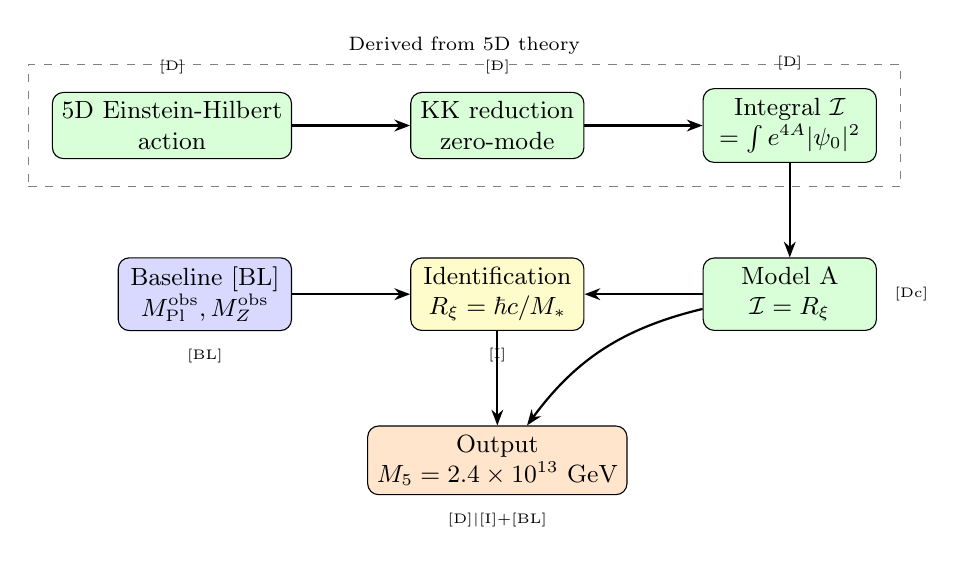
\begin{tikzpicture}[
    node distance=0.8cm,
    box/.style={rectangle, draw, rounded corners, minimum width=2.2cm,
                minimum height=0.7cm, align=center, font=\small},
    derived/.style={box, fill=green!15},
    identified/.style={box, fill=yellow!20},
    baseline/.style={box, fill=blue!15},
    output/.style={box, fill=orange!20},
    arrow/.style={-{Stealth[length=2mm]}, thick}
]

% Row 1: Axioms/Setup
\node[derived] (axioms) {5D Einstein-Hilbert\\action};
\node[derived, right=1.5cm of axioms] (reduction) {KK reduction\\zero-mode};
\node[derived, right=1.5cm of reduction] (integral) {Integral $\calI$\\$= \int e^{4A}|\psi_0|^2$};

% Row 2: Model choice and identification
\node[derived, below=1.2cm of integral] (modelA) {Model A\\$\calI = \Rxi$};
\node[identified, left=1.5cm of modelA] (identify) {Identification\\$\Rxi = \hbar c/M_*$};
\node[baseline, left=1.5cm of identify] (baseline) {Baseline [BL]\\$\Mpl^{\mathrm{obs}}, \MZ^{\mathrm{obs}}$};

% Row 3: Output
\node[output, below=1.2cm of identify] (M5) {Output\\$\Mfive = 2.4 \times 10^{13}$~GeV};

% Arrows
\draw[arrow] (axioms) -- (reduction);
\draw[arrow] (reduction) -- (integral);
\draw[arrow] (integral) -- (modelA);
\draw[arrow] (modelA) -- (identify);
\draw[arrow] (baseline) -- (identify);
\draw[arrow] (identify) -- (M5);
\draw[arrow] (modelA) to[bend right=20] (M5);

% Labels
\node[font=\tiny, above=0.1cm of axioms] {[D]};
\node[font=\tiny, above=0.1cm of reduction] {[D]};
\node[font=\tiny, above=0.1cm of integral] {[D]};
\node[font=\tiny, right=0.1cm of modelA] {\tiny[Dc]};
\node[font=\tiny, below=0.1cm of identify] {[I]};
\node[font=\tiny, below=0.1cm of baseline] {[BL]};
\node[font=\tiny, below=0.1cm of M5] {[D]$|$[I]+[BL]};

% Legend
\begin{scope}[on background layer]
\node[draw=gray, dashed, fit=(axioms)(reduction)(integral),
      inner sep=0.3cm, label={[font=\scriptsize]above:Derived from 5D theory}] {};
\end{scope}

\end{tikzpicture}
\caption{Gravity sector derivation pipeline. Green boxes: derived [D].
Yellow: identified [I]. Blue: baseline inputs [BL]. Orange: output.
\textbf{Schematic only; not to scale; no new results; consolidation of v13--v17.}}
\label{fig:pipeline}
\end{figure}

%═══════════════════════════════════════════════════════════════════════════════
\section{Epistemic Ledger}
%═══════════════════════════════════════════════════════════════════════════════

\begin{table}[h]
\centering
\caption{Complete epistemic ledger for BLOCK-003 gravity closure.}
\label{tab:ledger}
\begin{tabular}{@{}llcl@{}}
\toprule
Element & Formula/Value & Tag & Source \\
\midrule
Normalization extractor & $\Mpl^2 = \Mfive^3 \calI$ & [D] & v13 \\
Newton constant & $\GN = 1/(8\pi\Mfive^3\calI)$ & [D] & v13 \\
Integral (Model A) & $\calI = \Rxi$ & [Dc] & v14 \\
EW identification & $\Rxi = \hbar c / \MZ$ & [I] & v16 \\
Z mass input & $\MZ = 91.1876$~GeV & [BL] & PDG \\
Planck mass input & $\Mpl = 1.221 \times 10^{19}$~GeV & [BL] & CODATA \\
Closure formula & $\Mfive = \Mpl^{2/3}\Rxi^{-1/3}$ & [D] & v15 \\
Numerical result & $\Mfive = 2.41 \times 10^{13}$~GeV & [D]$|$[BL] & v16 \\
Robustness & $\Delta\log_{10}\Mfive < 0.15$ & [D] & v17 \\
Internal derivation & $\Rxi$ from axioms & \textbf{NO-GO} & v16 \\
\bottomrule
\end{tabular}
\end{table}

%═══════════════════════════════════════════════════════════════════════════════
\section*{Summary}
%═══════════════════════════════════════════════════════════════════════════════

\begin{center}
\fbox{\parbox{0.9\textwidth}{
\textbf{BLOCK-003 Gravity Sector Status:} \\[4pt]
\textbf{CLOSED (calibrated)} under minimal baseline inputs ($\Mpl^{\mathrm{obs}}$, $\MZ^{\mathrm{obs}}$). \\[4pt]
\textbf{NOT closed as pure prediction}: $\Rxi$ identification is [I]+[BL], not [D]. \\[4pt]
\textbf{Result}: $\Mfive = 2.41 \times 10^{13}$~GeV (GUT scale) $\pm 0.001\%$. \\[4pt]
\textbf{Robustness}: Verified across EW-scale family (v17). \\[4pt]
\textbf{Open item}: Internal derivation of $\Rxi$ remains NO-GO.
}}
\end{center}

\vspace{1em}
\noindent\textit{This document consolidates derivations v13--v17; no new results are claimed.}

\end{document}
